% ----------------------------------------------------------------------------------------------------- %
% Manual da Classe UFTeX
% 
% Versão 2.1:   Março 2018
%
% Criado por:   Tiago da Silva Almeida
% Revisado por: Tiago da Silva Almeida
%               Rafael Lima de Carvalho
%               Ary Henrique Morais de Oliveira
%
% https://almeidatiago.github.io/uftex/
% ----------------------------------------------------------------------------------------------------- %

\documentclass[report]{uftex}
% ---- Esse comando cria o nome uftex estilizado
\newcommand\uftex{UF\TeX}

\usepackage{lipsum}
\usepackage{tikz}
\usepackage[siunitx]{circuitikz}
\usetikzlibrary{arrows}

\usepackage[alf,abnt-emphasize=bf]{abntex2cite}
\renewcommand{\backrefpagesname}{}
\renewcommand{\backref}{}
\renewcommand*{\backrefalt}[4]{}
% ----  Esse comandos são necessário no pré-ambulo para a impressão da lista de lista abreviatuas e de símbolos
\makelosymbols
\makeloabbreviations
% ---- Início do documento
\begin{document}
  % ---- Descrição do título do trabalho 
  \title{Titulo do trabalho}
  % ---- Nome do autor ou autores do trabalho
  \author{Autor}{Sobrenome}
  \class{Sistemas Digitais}
  % ---- Nome do orientador do trabalho. O último campo representa o título do professor
  \advisor{Prof.}{Tiago}{da Silva Almeida}{Me.}
  % ---- Departamento representa o curso ao qual o trabalho está sendo apresentado. Descrito por meio de duas iniciais do curso
  \department{CC}
  % ---- Data da apresentação do trabalho
  \date{25}{03}{2016}
  % ---- Palavras-chaves em português do trabalho
  \keyword{\LaTeX}
  \keyword{\uftex}
  \keyword{Trabalho de Conclusão de Curso}
  \keyword{Redação Científica}
  \keyword{Extensão Universitária}
  % ---- Palavras-chaves em inglês do trabalho
  \foreignkeyword{\LaTeX}
  \foreignkeyword{\uftex}
  \foreignkeyword{Bachelor Thesis}
  \foreignkeyword{Scientific Writing}
  \foreignkeyword{University Extension}
  % ---- Comando responsável por criar a capa do trabalho e/ou folha de resto conforme a configuração exigida
  \maketitle

  \frontmatter

  \begin{abstract}
  \lipsum[1]
  \end{abstract}

  \begin{foreignabstract}
  \lipsum[9]
  \end{foreignabstract}
  \printlosymbols  
  \printloabbreviations
  % ---- Cria a lista de figuras. OPCIONAL
  %\listoffigures
  % ---- Cria a lista de tabelas. OPCIONAL
  %\listoftables 
  % ---- Cria o sumário. OBRIGATÓRIO
  \tableofcontents % sumário
% --- Marca o inicio dos elementos textuais. Capítulos.
\mainmatter
% ---- Defino o espaçamento de um e meio centímetros
\onehalfspacing
% ----------------------------------------------------------------------------------------------------- %
% Capítulos do trabalho
% ----------------------------------------------------------------------------------------------------- %
\ChapterStart{first}{First chapter}
\chapter{Introdução}

\lipsum[1] \cite{JW82} \symbl{$\phi$}{Definição do Símbolo 1} \symbl{$\Omega$}{Definição do Símbolo 2}

\lipsum[2] \cite{MenaChalco08} \abbrev{UFT}{Universidade Federal do Tocantins}\abbrev{CUP}{Campus Universitário de Palmas}

\lipsum[3] \cite{alves03:simi}

\section{Foo}

\subsection{Bar}

\citeonline{bobaoglu93:concepts} \lipsum[4]

\subsubsection{Foo}

\lipsum[5] \cite{bronevetsky02}

\lipsum[6] \cite{garcia01:PhD}

\lipsum[7] \cite{schmidt03:MSc}

\lipsum[8] \cite{alvisi99:analysisCIC}

\chapter{Métodos}

\section{Bar}

\lipsum[9] \cite{CORBA:spec}

\begin{eqnarray}
f(x) = \left\{
  \begin{array}{lr}
    x^2 & : x < 0\\
    x^3 & : x \ge 0
  \end{array}
\right.
\end{eqnarray}

\begin{eqnarray}
f(x) & = \int h(x)\, dx
\end{eqnarray}

\begin{eqnarray}
x = a_0 + \frac{1}{a_1 + \frac{1}{a_2 + \frac{1}{a_3 + a_4}}}
\end{eqnarray}

\begin{eqnarray}
\prod_{1\le i \le n}
     M_{i,j}
\end{eqnarray}

\lipsum[10] \cite{gridftp}

\subsection{Foo}

\begin{lstlisting}[language=C]
#include<stdio.h>
#include<iostream>
    // A comment
int main(void) {
    printf("Hello World\n");
    return 0;
}
\end{lstlisting}

\begin{lstlisting}[language=Java]
public class HelloWorld {
   public static void main(String[] args) {
      // Prints "Hello, World" in the terminal window.
      System.out.println("Hello, World");
   }
}
\end{lstlisting}

\begin{lstlisting}[language=Python]
x = 1
if x == 1:
    # indented four spaces
    print("x is 1.")
\end{lstlisting}

\subsubsection{Bar}

\lipsum[11] \cite{fowler04:designDead}

\begin{table}[!htpb]
\centering
\caption{xxxx.}\label{tab:tab1}
   \begin{tabular}{ | l | l | l | p{5cm} |}
    \hline
    Day & Min Temp & Max Temp & Summary \\ \hline
    Monday & 11C & 22C & A clear day with lots of sunshine.  
    However, the strong breeze will bring down the temperatures. \\ \hline
    Tuesday & 9C & 19C & Cloudy with rain, across many northern regions. Clear spells 
    across most of Scotland and Northern Ireland, 
    but rain reaching the far northwest. \\ \hline
    Wednesday & 10C & 21C & Rain will still linger for the morning. 
    Conditions will improve by early afternoon and continue 
    throughout the evening. \\
    \hline
    \end{tabular}
\end{table}

\lipsum[12] \cite{FSF:GNU-GPL}

\begin{table}[!htpb]
\centering
\caption{xxxx.}\label{tab:tab1}
\begin{tabular}{l*{6}{c}r}
Team              & P & W & D & L & F  & A & Pts \\
\hline
Manchester United & 6 & 4 & 0 & 2 & 10 & 5 & 12  \\
Celtic            & 6 & 3 & 0 & 3 &  8 & 9 &  9  \\
Benfica           & 6 & 2 & 1 & 3 &  7 & 8 &  7  \\
FC Copenhagen     & 6 & 2 & 1 & 3 &  5 & 8 &  7  \\
\end{tabular}
\end{table}

\lipsum[13] \cite{eco:09}

\begin{table}[!htpb]
\centering
\caption{xxxx.}\label{tab:tab1}
\begin{tabular}{ |l|l|l| }
\hline
\multicolumn{3}{ |c| }{Team sheet} \\
\hline
Goalkeeper & GK & Paul Robinson \\ \hline
\multirow{4}{*}{Defenders} & LB & Lucas Radebe \\
 & DC & Michael Duburry \\
 & DC & Dominic Matteo \\
 & RB & Didier Domi \\ \hline
\multirow{3}{*}{Midfielders} & MC & David Batty \\
 & MC & Eirik Bakke \\
 & MC & Jody Morris \\ \hline
Forward & FW & Jamie McMaster \\ \hline
\multirow{2}{*}{Strikers} & ST & Alan Smith \\
 & ST & Mark Viduka \\
\hline
\end{tabular}
\end{table}

\lipsum[14] \cite{zobel:04}

\chapter{Resultados}

\lipsum[15] \cite{waz:09}

\begin{figure}[!htpb]
\centering
\caption{zzzzzzzz.}\label{fig:fig1}
\begin{circuitikz}
	\draw
	% Drawing a npn transistor
	(0,0) node[npn](npn1){} 
	% Making connections from transistor using relative coordinates
	(npn1.E) node[right=7mm, above=5mm]{2N2222} % Labelling the transistor
	(npn1.B) -- ++(-1,0) to [R,l_=10<\kilo\ohm>,*-*] ++(0,-3)  
	(npn1.B) -- ++(-3,0) to [C,l_=100<\nano\farad>] ++(0,-3) node(gnd1){}
	(npn1.E) to [R,l_=10<\kilo\ohm>,*-*] (0,-3)
	(npn1.E) -- ++(2,0) to [C,l=10<\pico\farad>,*-*] (2,-3)
	(npn1.B) -- ++(-1,0) to [R,l_=10<\kilo\ohm>,*-] ++(0,3) node(con1){}
	(npn1.C) to [L,l_=150<\micro\henry>,*-] (0,3) 
	(npn1.C) -- ++(2,0) to [C,l=10<\pico\farad>,*-*] ++(0,-1.5)
	% Drawing shorts and ground connection
	(-1,3)to[short,*-o] (-1,4) node[right]{$V_{DD}=6 VDC$} % Power supply
	% Output sinusoidal waveform at approximately 50 MHz
	(npn1.C) -- ++(4,0) to [short,-o]
	  ++(0,0) node[right]{$V_o (\approx \SI{50}{\MHz})$}
	(0,-3) node[ground]{}% Define this node as ground
	(gnd1) ++(0,0) to[short,-o] ++(7.85,0)
        (con1)to[short] ++(1.85,0)
	;
\end{circuitikz}
\end{figure}

\lipsum[16] \cite{Higham:98}

\begin{figure}[!htpb]
\centering
\caption{zzzzzzzz.}\label{fig:fig1}
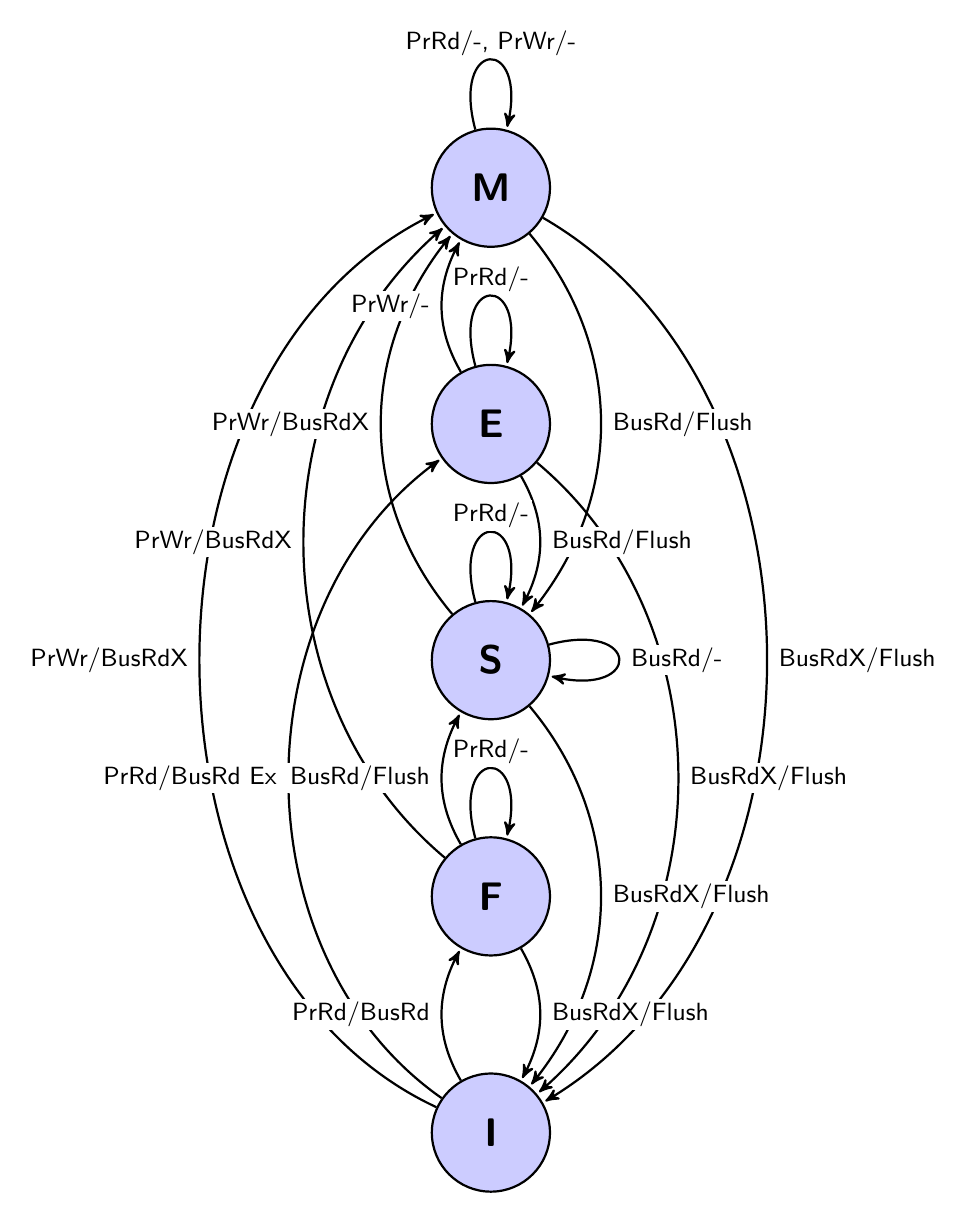
\begin{tikzpicture}[->,>=stealth',shorten >=1pt,auto,node distance=3cm,
  thick,main node/.style={circle,fill=blue!20,draw,
  font=\sffamily\Large\bfseries,minimum size=15mm}]

  \node[main node] (M) {M};
  \node[main node] (E) [below of=M] {E};
  \node[main node] (S) [below of=E] {S};
  \node[main node] (F) [below of=S] {F};
  \node[main node] (I) [below of=F] {I};

  \path[every node/.style={font=\sffamily\small,
  		fill=white,inner sep=1pt}]
  	% Right-hand-side arrows rendered from top to bottom to
  	% achieve proper rendering of labels over arrows.
    (M) edge [loop above] node {PrRd/-, PrWr/-} (M)
        edge [bend left=60] node[right=1mm] {BusRdX/Flush} (I)
        edge [bend left=40] node[right=1mm] {BusRd/Flush} (S)
    (E) edge [loop above] node {PrRd/-} (E)
        edge [bend left=50] node[right=1mm] {BusRdX/Flush} (I)
        edge [bend left=30] node[right=1mm] {BusRd/Flush} (S)
    (S) edge [loop above] node {PrRd/-} (S)
        edge [loop right] node[right=1mm]  {BusRd/-} (S)
        edge [bend left=40] node[right=1mm] {BusRdX/Flush} (I)
    (F) edge [bend left=30] node[right=1mm] {BusRdX/Flush} (I)
        
  	% Left-hand-side arrows rendered from bottom to top to
  	% achieve proper rendering of labels over arrows.
    (I) edge [bend left=65] node[left=1mm] {PrWr/BusRdX} (M)
        edge [bend left=55] node[left=1mm] {PrRd/BusRd Ex} (E)
        edge [bend left=30] node[left=1mm] {PrRd/BusRd} (F)
    (F) edge [loop above] node {PrRd/-} (F)
        edge [bend left=50] node[left=1mm] {PrWr/BusRdX} (M)
        edge [bend left=30] node[left=1mm] {BusRd/Flush} (S)
    (S) edge [bend left=40] node[left=1mm] {PrWr/BusRdX} (M)
    (E) edge [bend left=30] node[left=1mm] {PrWr/-} (M);
\end{tikzpicture}
\end{figure}

\lipsum[17] \cite{Knuth:96}

\begin{figure}[!htpb]
\centering
\caption{zzzzzzzz.}\label{fig:fig1}
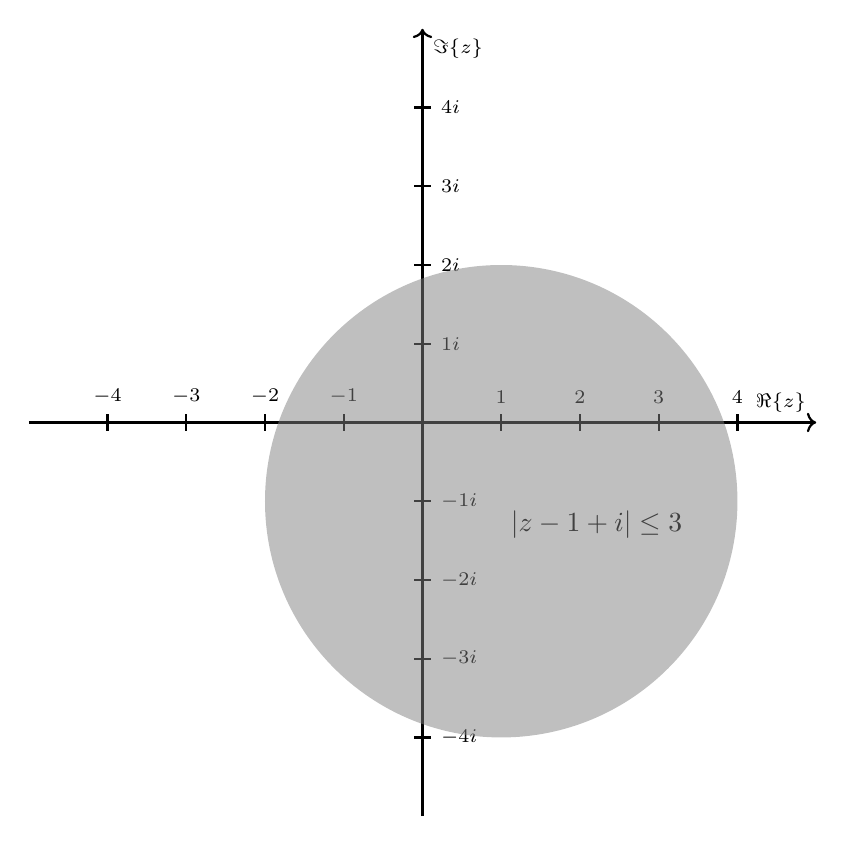
\begin{tikzpicture}
    \begin{scope}[thick,font=\scriptsize]
    % Axes:
    % Are simply drawn using line with the `->` option to make them arrows:
    % The main labels of the axes can be places using `node`s:
    \draw [->] (-5,0) -- (5,0) node [above left]  {$\Re\{z\}$};
    \draw [->] (0,-5) -- (0,5) node [below right] {$\Im\{z\}$};

    % Axes labels:
    % Are drawn using small lines and labeled with `node`s. The placement can be set using options
    \iffalse% Single
    % If you only want a single label per axis side:
    \draw (1,-3pt) -- (1,3pt)   node [above] {$1$};
    \draw (-1,-3pt) -- (-1,3pt) node [above] {$-1$};
    \draw (-3pt,1) -- (3pt,1)   node [right] {$i$};
    \draw (-3pt,-1) -- (3pt,-1) node [right] {$-i$};
    \else% Multiple
    % If you want labels at every unit step:
    \foreach \n in {-4,...,-1,1,2,...,4}{%
        \draw (\n,-3pt) -- (\n,3pt)   node [above] {$\n$};
        \draw (-3pt,\n) -- (3pt,\n)   node [right] {$\n i$};
    }
    \fi
    \end{scope}
    % The circle is drawn with `(x,y) circle (radius)`
    % You can draw the outer border and fill the inner area differently.
    % Here I use gray, semitransparent filling to not cover the axes below the circle
    \path [draw=none,fill=gray,semitransparent] (+1,-1) circle (3);
    % Place the equation into the circle:
    \node [below right,darkgray] at (+1,-1) {$|z-1+i| \leq 3$};
\end{tikzpicture}
\end{figure}

\backmatter 
\singlespacing   
% ----------------------------------------------------------------------------------------------------- %
\bibliography{relatorio_exemplo}

\appendix
\onehalfspacing

\chapter{Sequências}
\label{ape:sequencias}

\lipsum[7]


\end{document}
